% Options for packages loaded elsewhere
\PassOptionsToPackage{unicode}{hyperref}
\PassOptionsToPackage{hyphens}{url}
%
\documentclass[
]{article}
\usepackage{amsmath,amssymb}
\usepackage{lmodern}
\usepackage{iftex}
\ifPDFTeX
  \usepackage[T1]{fontenc}
  \usepackage[utf8]{inputenc}
  \usepackage{textcomp} % provide euro and other symbols
\else % if luatex or xetex
  \usepackage{unicode-math}
  \defaultfontfeatures{Scale=MatchLowercase}
  \defaultfontfeatures[\rmfamily]{Ligatures=TeX,Scale=1}
\fi
% Use upquote if available, for straight quotes in verbatim environments
\IfFileExists{upquote.sty}{\usepackage{upquote}}{}
\IfFileExists{microtype.sty}{% use microtype if available
  \usepackage[]{microtype}
  \UseMicrotypeSet[protrusion]{basicmath} % disable protrusion for tt fonts
}{}
\makeatletter
\@ifundefined{KOMAClassName}{% if non-KOMA class
  \IfFileExists{parskip.sty}{%
    \usepackage{parskip}
  }{% else
    \setlength{\parindent}{0pt}
    \setlength{\parskip}{6pt plus 2pt minus 1pt}}
}{% if KOMA class
  \KOMAoptions{parskip=half}}
\makeatother
\usepackage{xcolor}
\usepackage[margin=1in]{geometry}
\usepackage{graphicx}
\makeatletter
\def\maxwidth{\ifdim\Gin@nat@width>\linewidth\linewidth\else\Gin@nat@width\fi}
\def\maxheight{\ifdim\Gin@nat@height>\textheight\textheight\else\Gin@nat@height\fi}
\makeatother
% Scale images if necessary, so that they will not overflow the page
% margins by default, and it is still possible to overwrite the defaults
% using explicit options in \includegraphics[width, height, ...]{}
\setkeys{Gin}{width=\maxwidth,height=\maxheight,keepaspectratio}
% Set default figure placement to htbp
\makeatletter
\def\fps@figure{htbp}
\makeatother
\setlength{\emergencystretch}{3em} % prevent overfull lines
\providecommand{\tightlist}{%
  \setlength{\itemsep}{0pt}\setlength{\parskip}{0pt}}
\setcounter{secnumdepth}{-\maxdimen} % remove section numbering
\usepackage[width=\textwidth]{caption}
\usepackage{wrapfig}
\ifLuaTeX
  \usepackage{selnolig}  % disable illegal ligatures
\fi
\IfFileExists{bookmark.sty}{\usepackage{bookmark}}{\usepackage{hyperref}}
\IfFileExists{xurl.sty}{\usepackage{xurl}}{} % add URL line breaks if available
\urlstyle{same} % disable monospaced font for URLs
\hypersetup{
  pdftitle={AIM Field Methods},
  hidelinks,
  pdfcreator={LaTeX via pandoc}}

\title{AIM Field Methods}
\author{}
\date{\vspace{-2.5em}}

\begin{document}
\maketitle

The Assess, Inventory, and Monitor program collects quantitative data
related to six core indicators of rangeland health. These indicators
were selected by the Bureau of Land Management as they respond quickly
to different management actions and are easy to interpret. The four
field methods utilized to collect these data, are relatively quick to
perform, can be learned quickly, and give repeatable measurements. Three
of these methods have been widely employed in the natural sciences for
over half a century, and the soil stability test was largely developed
around the millennium by researchers whom went on to develop AIM.

\begin{wraptable}{l}{90mm}
    \begin{tabular}{c | c}
      \textbf{Indicator} & \textbf{Method}\\ \hline
      Cover Bare Ground & Line-Point Intercept (LPI) \\ \hline
      Vegetation Composition & Line-Point Intercept (LPI) \\ \hline
      Vegetation Height & (LPI) + Height \\ \hline
      Length of Bare-ground & Line-Intercept ('Gap Intercept')  \\ \hline
      Invasive Species & Species Richness; LPI \\ \hline
      Soil Aggregate Stability & Soil Stability \\ \hline
    \end{tabular}
    \caption{Variables used to Calculate Potential Evaporation}
    \label{Potential Evaporation}
\end{wraptable}

\hypertarget{species-inventory}{%
\subsection{Species Inventory}\label{species-inventory}}

The entirety of an AIM plot, a circle with 30m radius and
\textasciitilde2700 m\textsuperscript{2}, is used to record the presence
of plant species. This area is wandered in a zig-zag fashion as the
technician records the presence of each vascular plant species they
encounter, and flag unknown species, for 15 minutes. In the event that
the technician is still detecting un-recorded species on the plot at
that point, they add an additional 2 minutes, until they cannot detect
another species in that interval. Species are then identified in field,
or from collected specimens.

\hypertarget{gap-intercept}{%
\subsection{Gap Intercept}\label{gap-intercept}}

The original formulation of this approach, \textbf{Line Intercept}, were
developed in the 1940's in order to sample shrublands in an effective
manner @canfield1941application, @bauer1943statistical. The commonly
used formulation of Line Intercept is able to quickly determine the
percent cover of physiognomically dominant shrubs such as Sagebrush. In
the Gap Intercept utilization, rather than measuring plants, the start
and end positions of bare ground are measured; it can considered the
inverse of the more common method.

AIM crews gather the total length of bare ground at three 25m transects,
in a tri-spoke design. Each line is orientated 120° from the others, and
emanating out from a `trample/sacrifice zone' an area at the center of a
plot which is prone to damage and giving erroneous measures. The
technician slowly walks the length of each transect, recording the
`Start' of bare soil, and the `End' of bare soil, for each gap
\textgreater{} 20cm in length. The bare soil `End', can be caused by
live or dead vegetation, or embedded plant debris
\textgreater\textasciitilde{} 2 mm in diameter.

\hypertarget{line-point-intercept}{%
\subsection{Line-Point Intercept}\label{line-point-intercept}}

The `point' part of this method was developed in New Zealand in the
early 1920's, the decision to align points along a line was developed
and popularized in the 1950's (@goodall1952some). Essentially, one has a
transect tape - a line, and has a predetermined number of locations they
will record the presence of a species at, generally these locations will
be equi-distant from each other.

AIM crews gather information at 150 points across the plot\ldots{}

\hypertarget{soil-stability}{%
\subsection{Soil Stability}\label{soil-stability}}

This method was developed in the late 90's in order to approximate the
susceptibility of soil to erosion (@CITE). It measures soil aggregates

\begin{wrapfigure}{r}{0.5\textwidth}
  \centering
    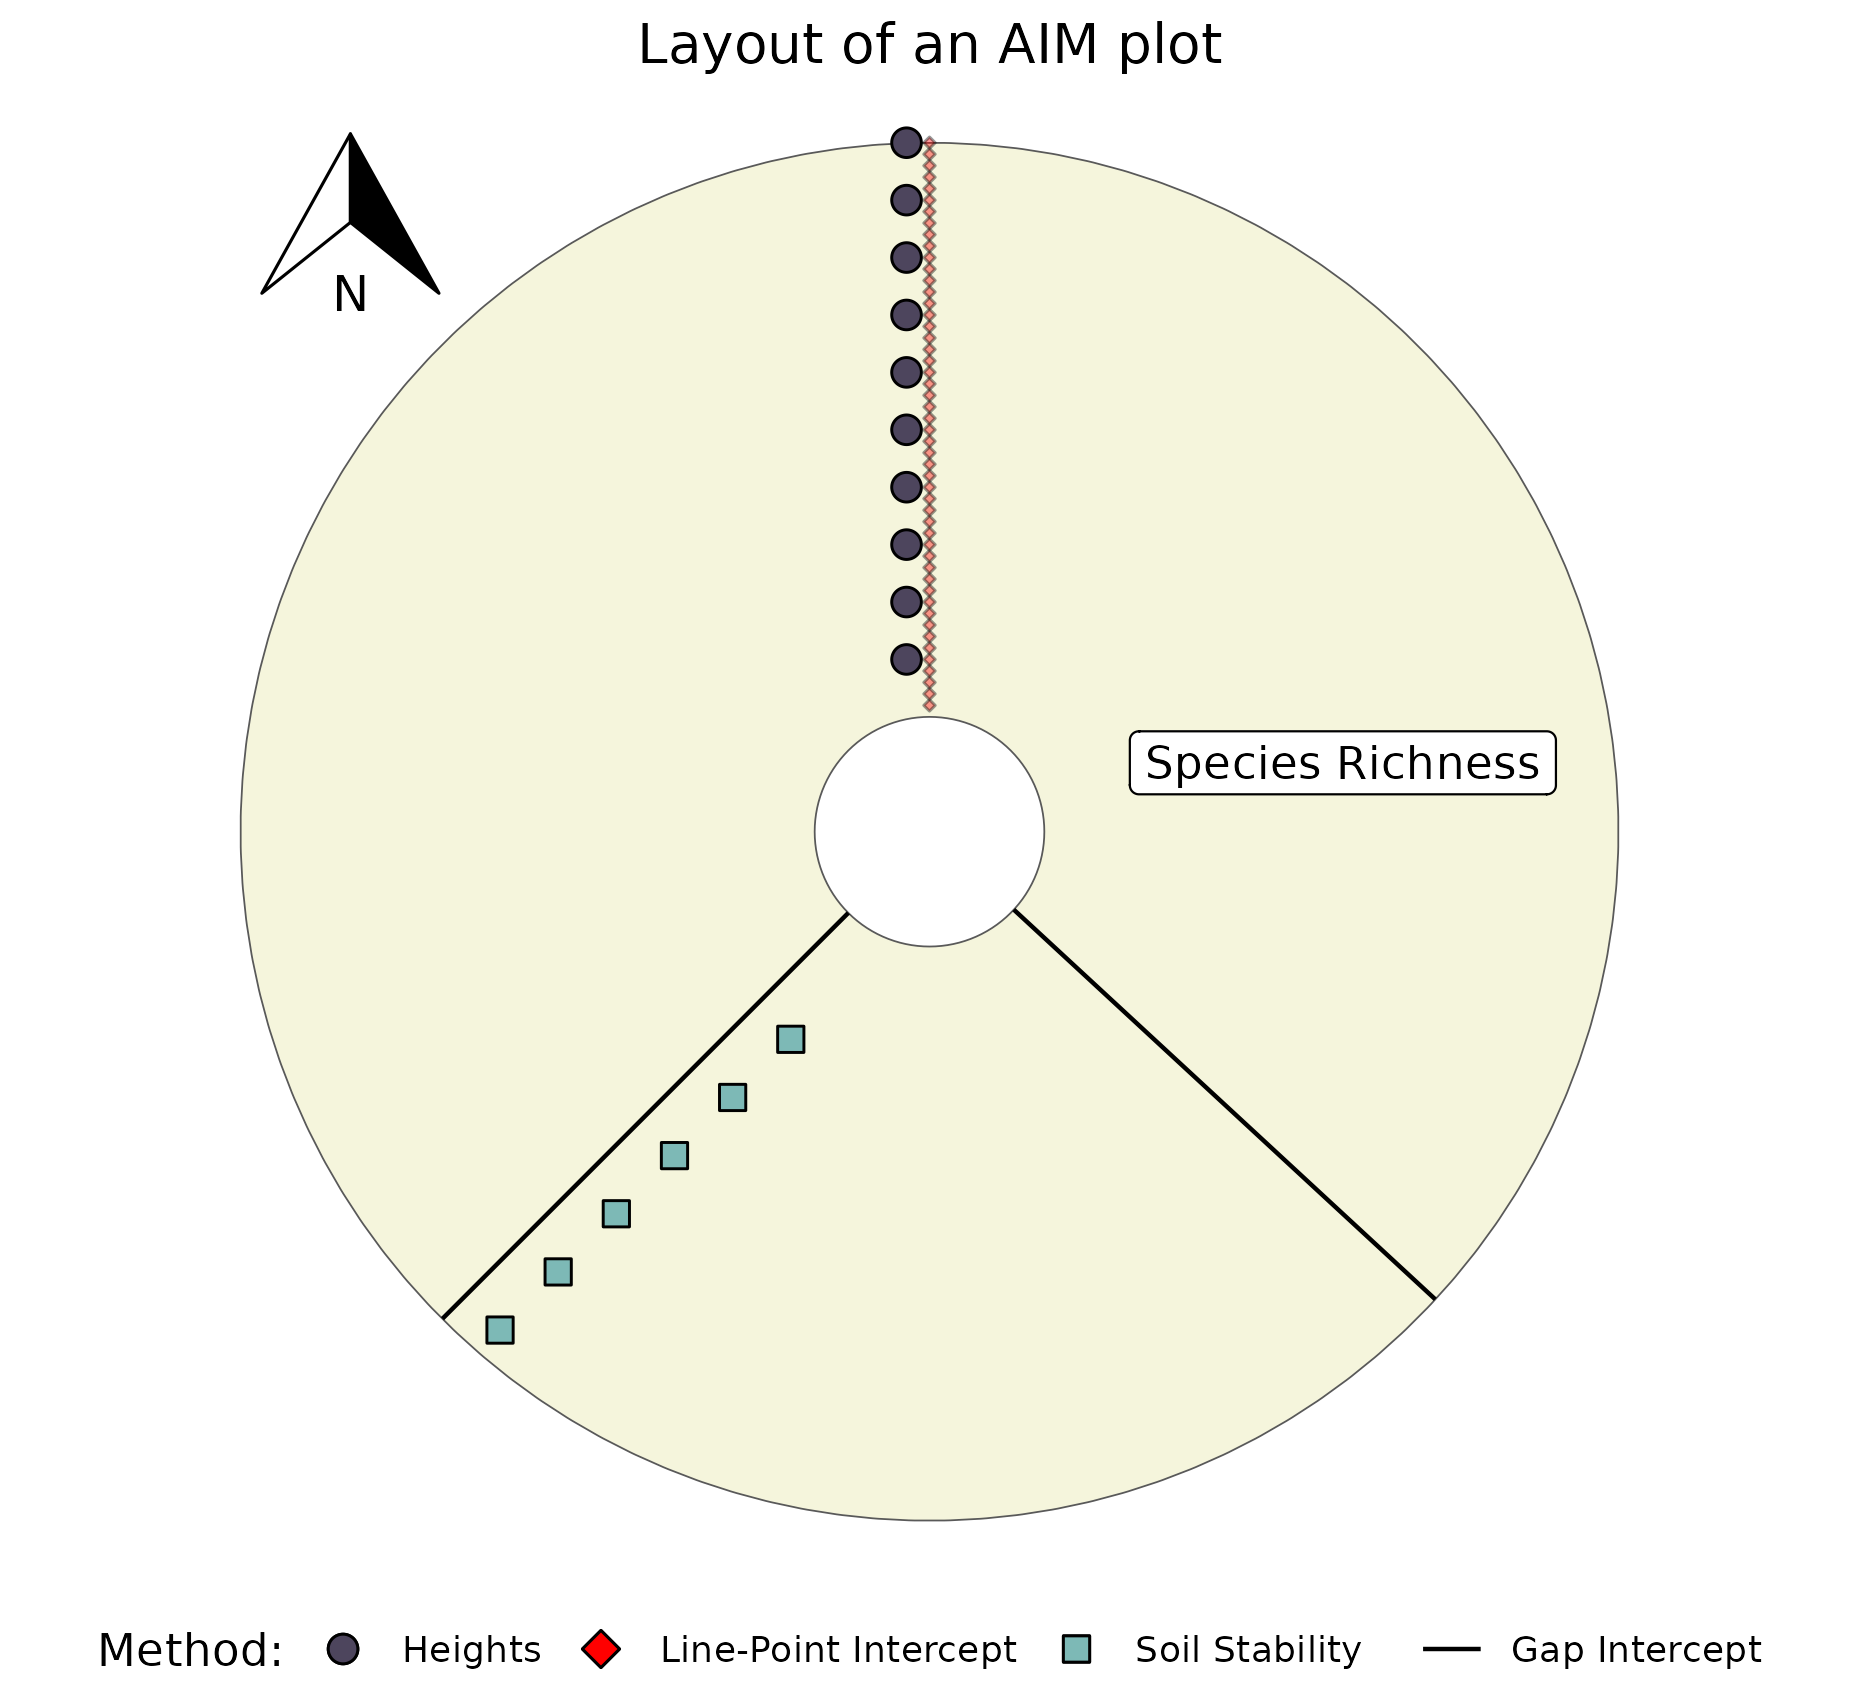
\includegraphics[width=0.5\textwidth]{../plots/graphics/Methods-Plot.png}
  \caption{Example AIM plot, with locations of the four major methods illustrated.}
\end{wrapfigure}

\end{document}
